\documentclass[handout]{beamer}
% \documentclass{beamer}

%%
%%
%%
% From http://tex.stackexchange.com/questions/2072/beamer-navigation-circles-without-subsections
% Solution #2 or 3:
% \usepackage{etoolbox}
% \makeatletter
% % replace the subsection number test with a test that always returns true
% \patchcmd{\slideentry}{\ifnum#2>0}{\ifnum2>0}{}{\@error{unable to patch}}%
% \makeatother
% Solution #1:
\usepackage{remreset}% tiny package containing just the \@removefromreset command
\makeatletter
\@removefromreset{subsection}{section}
\makeatother
\setcounter{subsection}{1}


\usepackage{etex}
\usepackage{pgf}
\usepackage{tikz}
\usepackage{url}
\usepackage{amsmath}
\usepackage{color}
% \definecolor{red}{rgb}{1,0,0}
\usepackage{ulem}
% \usepackage{booktabs}
\usepackage{colortbl,booktabs}
\renewcommand*{\thefootnote}{\fnsymbol{footnote}}
\usepackage{fancybox}
\usepackage[framemethod=TikZ]{mdframed}
\mdfdefinestyle{FactStyle}{%
  outerlinewidth=0.5,
  roundcorner=1pt,
  leftmargin=1cm,
  linecolor=blue,
  outerlinecolor=blue!70!black,
  backgroundcolor=yellow!40
}
\usepackage{cancel}

  \newcommand\Warning{%
    \makebox[2.4em][c]{%
      \makebox[0pt][c]{\raisebox{.2em}{\Large!}}%
      \makebox[0pt][c]{\color{red}\Huge$\bigtriangleup$}}}%

\usepackage{stackengine}
\usepackage{scalerel}
\usepackage{xcolor}
  \newcommand\dangersign[1][2ex]{%
    \renewcommand\stacktype{L}%
    \scaleto{\stackon[1.3pt]{\color{red}$\triangle$}{\tiny !}}{#1}%
  }



\usepackage{dcolumn}
\newcolumntype{d}[1]{D{.}{.}{#1}}

% From
% http://tex.stackexchange.com/questions/109900/how-can-i-box-multiple-aligned-equations
\usepackage{empheq}
\usepackage{tcolorbox}  \newtcbox{\othermathbox}[1][]{%
  nobeforeafter, tcbox raise base, 
  colback=black!10, colframe=red!30, 
  left=1em, top=0.5em, right=1em, bottom=0.5em}

\newcommand\blue{\color{blue}}
\newcommand\red{\color{red}}
\newcommand\green{\color{green!75!black}}
\newcommand\purple{\color{purple}}
\newcommand\bluegreen{\color{blue!75!green}}
\newcommand\orange{\color{orange}}
\newcommand\redgreen{\color{red!50!green}}
\newcommand\grey{\color{black}}
\newcommand\gap{\vspace{.1in}}
\newcommand\nb{${\red\bullet}\ $}
\newcommand\halfgap{\vspace{.05in}}
\newcommand\divideline{\line(1,0){352}}
\usepackage{marvosym} % for \Smiley

\newcommand{\bluealert}[1]{{\blue\textbf{#1}}}

% \usepackage{beamerthemesplit} %Key package for beamer
\usetheme{Singapore}
% \usetheme{Szeged}
% \usetheme{Garfield}
% \usetheme{CambridgeUS}
% \usenavigationsymbolstemplate{} %Gets rid of slide navigation symbols


\setbeamercolor{separation line}{use=structure,bg=structure.fg!50!bg}
% \begin{beamercolorbox}[colsep=0.5pt]
%   {upper separation line foot}
% \end{beamercolorbox}



\makeatletter
\setbeamertemplate{footline}
{
  \leavevmode%
  \hbox{%
% \begin{beamercolorbox}[colsep=0.5pt]
%   {upper separation line foot}
% \end{beamercolorbox}


  \begin{beamercolorbox}[wd=.5\paperwidth,ht=2.25ex,dp=2ex,colsep=0.5pt]%
    {upper separation line foot}
    \usebeamerfont{author in head/foot}%
    \hspace*{2ex}\insertshortdate:\ \insertshorttitle
  \end{beamercolorbox}%
  \begin{beamercolorbox}[wd=.5\paperwidth,ht=2.25ex,dp=2ex,right]{title in head/foot}%
    \usebeamerfont{title in head/foot}
    {\insertshortauthor}\hspace*{2ex}
  \end{beamercolorbox}}%
  % \begin{beamercolorbox}[wd=.333333\paperwidth,ht=2.25ex,dp=2ex,right]{date in head/foot}%
  %   \usebeamerfont{date in head/foot}\insertshortdate{}\hspace*{2em}
  %   \insertframenumber{} / \inserttotalframenumber\hspace*{2ex} 
  % \end{beamercolorbox}%
  \vskip0pt%
}
\makeatother

\usetikzlibrary{decorations.markings}
\usetikzlibrary{arrows}


\title{Final Exam Review}
\author{Peter Garfield, UCSB Mathematics}
\date{March 15, 2017}
%\institute{}


\useinnertheme{default}

\usefonttheme{serif}
% \usecolortheme{rose}
% \usecolortheme{whale}
% \usecolortheme{orchid}
\usecolortheme{crane}
% \usecolortheme{dolphin}


%TEMPLATE
\setbeamertemplate{navigation symbols}{}

\setbeamertemplate{note page}[compress]

\setbeamertemplate{frametitle}{
  \vspace{0.5em}
  % \begin{centering}
  {\huge\blue\textbf{\textmd{\insertframetitle}}}
  \par
  % \end{centering}
}

% From http://tex.stackexchange.com/questions/7032/good-way-to-make-textcircled-numbers:
\newcommand*\circled[1]{\tikz[baseline=(char.base)]{\node[shape=circle,draw,fill=orange,inner sep=1pt] (char) {#1};}} 
% \renewcommand{\labelenumi}{\circled{\textbf{\arabic{enumi}}}}

\let\olddescription\description
\let\oldenddescription\enddescription
\usepackage{enumitem}
\let\description\olddescription
\let\enddescription\oldenddescription

% \usepackage[loadonly]{enumitem}
\setlist[enumerate,1]{label=\colorbox{orange}{\arabic*.},font=\bfseries}
%\setlist[enumerate,2]{label=\colorbox{blue!25}{(\alph*)},font=\bfseries}
% \setlist[enumerate,1]{label=\arabic*.,font=\bfseries}
\setlist[itemize,1]{label=\red$\bullet$}
\setlist[itemize,2]{label=\blue$\bullet$}

\newcommand\answer[1]{\fbox{#1}}
% \renewcommand\answer[1]{}

\newcommand{\antilog}{\operatorname{antilog}}







\title{}
\title{Logs in Different Bases; Review}
\date{May 5, 2017}


\begin{document}
\small

\section*{Administration}

\frame{
  \frametitle{Office Hours!}
  % \ \vspace*{0.25in}

  {\Large{}Instructor:}\\
  \ \hspace*{0.2in} Peter M.\ Garfield, \url{garfield@math.ucsb.edu}\\[0.25em]

  {\Large{}Office Hours:}\\
  \ \hspace*{0.2in} Mondays 2--3\textsc{pm}\\
  \ \hspace*{0.2in} Tuesdays 10:30--11:30\textsc{am}\\
  \ \hspace*{0.2in} Thursdays 1--2\textsc{pm}\\
  \ \hspace*{0.2in} or by appointment \\[0.25em]

  {\Large{}Office:}\\
  \ \hspace*{0.2in} South Hall 6510\\[0.5em]

  \copyright\ 2017\ Daryl Cooper, Peter M.\ Garfield

  % \vspace*{2in}
}

\section*{Log Review}

\frame{
  \frametitle{Summary of Logs}

  $\log(y)$ is {\blue how many tens you multiply together to get $y$}.
  \bigskip

  \begin{minipage}{0.4\linewidth}
    \begin{empheq}[box=\othermathbox]{align*}
      10^{\log(y)} = y
    \end{empheq}
  \end{minipage}
  \hspace*{0.25in}
  \begin{minipage}{0.4\linewidth}
    \begin{empheq}[box=\othermathbox]{align*}
      \log\left( 10^a \right) = a
    \end{empheq}
  \end{minipage}
  \bigskip
  \pause

  \begin{minipage}{0.4\linewidth}
    \begin{empheq}[box=\othermathbox]{align*}
      10^{a} {\red\times} 10^b = 10^{a{\red+}b}
    \end{empheq}
  \end{minipage}
  \hspace*{0.25in}
  \begin{minipage}{0.4\linewidth}
    \begin{empheq}[box=\othermathbox]{align*}
      \log(x{\red\times}y) = \log(x) {\red+} \log(y)
    \end{empheq}
  \end{minipage}
  \bigskip
  \pause

  \begin{minipage}[b]{0.4\linewidth}
    \begin{empheq}[box=\othermathbox]{align*}
      \left( 10^{a} \right)^{\red{}p} = 10^{a{\red{}p}}
    \end{empheq}
  \end{minipage}
  \hspace*{0.25in}
  \begin{minipage}[b]{0.4\linewidth}
    \begin{empheq}[box=\othermathbox]{align*}
      \log(a^{\,\red{}p}) = {\red{}p}\log(a)
    \end{empheq}
  \end{minipage}
  \bigskip

  \pause
  {\red{}Each of these pairs of equalities says one thing!}


}

\section*{Other Bases}

\frame{
  \frametitle{\S7.13: Logs in Other Bases}

  $\log(y)$ is {\blue how many tens you multiply together to get $y$}.
  \bigskip

  \uncover<2->{%
    $\log_2(y)$ is {\blue how many {\red{}twos}\ you multiply together to get $y$}.
    \bigskip
  }

  \uncover<3->{%
    So ${\orange2}^{\red 3}={\blue 8} \qquad\text{means the same thing as}\qquad\log_{{\orange2}}({\blue 8})={\red 3}$
    \gap
    \pause
  }

  \uncover<4->{%
    \alert{Examples:}
  }
  \begin{align*}
    \uncover<4->{\log_{{\redgreen2}}({\blue 16})
    & = }
      \uncover<5->{%
      {\red 4}
    && \text{because}\ {\redgreen2}^{\red 4}={\blue 16} \\
    \log_{{\redgreen2}}({\blue 32})
    & = }
      \uncover<6->{%
      {\red 5}
    &&\text{because}\ {\redgreen2}^{\red 5}={\blue 32}\\
    \log_{{\redgreen2}}({\blue 1/8})
    & = }
      \uncover<7->{%
      {\red -3}
    && \text{because}\ {\redgreen2}^{\red -3}={\blue 1/8}
       }
  \end{align*}

  \uncover<8->{%
    The five laws of logs work {\blue for any base} {\red b}\
    exactly the same way except\ldots
  }

  \uncover<9->{%
    \begin{minipage}{0.4\linewidth}
      \begin{empheq}[box=\othermathbox]{align*}
        {\red{}b}^{\log_{\red{}b}(y)} = y
      \end{empheq}
    \end{minipage}
    \hspace*{0.25in}
    \begin{minipage}{0.4\linewidth}
      \begin{empheq}[box=\othermathbox]{align*}
        \log_{\red{}b}\left( {\red{}b}^a \right) = a
      \end{empheq}
    \end{minipage}
  }

}

\frame{
  \frametitle{Summary \& Examples}

  \alert{Important bases:}
  \begin{itemize}
  \item $\log_{\red2}$ is used extensively in computer science
  \item $\ln = \log_{\red{}e}$ is used everywhere (the {\red{}natural log})
    ($e\approx2.718$) \\
    \pause
    $\log_{\red e}({\blue y})={\redgreen x}$ means ${\red e}^{\redgreen x}={\blue y}$
    \\ \pause
    $\log_{\red e}({\blue y})$ is how many ${\red e}$'s you multiply to get ${\blue y}$.
    \\ \pause
    Read as: `` log base ${\red e}$ of ${\blue y}$ equals ${\redgreen x}$.''
  \end{itemize}
  \pause
  \gap 

  \alert{Examples:}
  \smallskip

  $\log_{\red 3}({\blue 81})=$
  \vspace*{-1.85em}

  \begin{center}
    A$=0$
    \quad 
    B$=1$
    \quad 
    C$=2$
    \quad 
    D$=3$
    \quad 
    E$=4$
    \pause
    \quad
    \fbox{E} 
  \end{center}
  \gap

  $\log_{\red 5}({\blue 25})=$
  \vspace*{-1.85em}

  \begin{center}
    A$=0$
    \quad 
    B$=1$
    \quad 
    C$=2$
    \quad 
    D$=3$
    \quad 
    E$=4$
    \pause
    \quad
    \fbox{C}
  \end{center}
  \halfgap

  Simplify $\ln\left(\left(e^{3x}\times e^{y}\right)^2\right)$
  \begin{center}
    A$=6x+ y$
    \quad 
    B$ = 2x+2y$
    \quad 
    C$ = 3x+2y$
    \quad 
    D$ = 6x+2y$
    \quad 
    E$=6xy$
    \quad 
    \pause
    \fbox{D}
  \end{center}
  \pause

  Teaser: $e$ is special because the derivative of $e^x$ is $e^x$
  \pause
  \ whatever that means.


}

\section*{Review}

\frame{
  \frametitle{Review Question \#1}

  If the price of an airplane ticket is $\$300$, then the airline
  sells $2,000$\ tickets.  For {\blue each dollar}\ the airline
  increases the price, it {\blue sells $10$ fewer tickets}.
  \gap

  \begin{itemize}
  \item[\red(1)] 
    If the price is $\$400$, how many tickets does the airline sell?
    \begin{center}
      A$=2000$
      \quad 
      B$= 1000$
      \quad 
      C$= 3000$
      \quad 
      D$= 1990$
      \quad 
      E$= 2400$
      \pause
      \quad
      \fbox{B}
    \end{center}
    \bigskip

    \item[\red(2)]
      If the price is \$$(300+{\blue n})$, how many tickets does
      the airline sell? 
      \begin{center}
        A$=2000-{\blue n}$
        \quad 
        B$= 2000+10{\blue n}$
        \quad 
        C$= 2000-10{\blue n}$
        \quad 
        D$ = 2000/{\blue n}$
        \pause
        \quad
        \fbox{C}
      \end{center}
      \bigskip

    \item[\red(3)]
      If the price is \$${\red x}$, how many tickets does the airline sell?
      \begin{center}
        A$=2000+10{\red x}$
        \quad 
        B$= 2000-10{\red x}$
        \quad 
        C$= 5000-10{\red x}$
        \quad 
        D$= 1000+10{\red x}$
        \pause
        \quad
        \fbox{C}
      \end{center}
      \bigskip
  \end{itemize}

}


\if0
\frame{
  \frametitle{Review Question \#2\ (HW13 \#9)}
  \vspace*{-1em}

  \begin{center}
    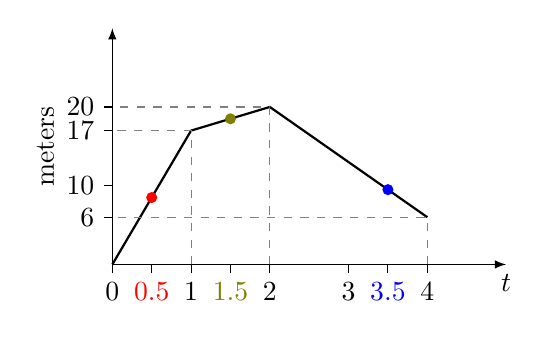
\begin{tikzpicture}[x=10mm,y=1mm,>=latex]
      \draw[thin,black,->] (0,0) -- (5,0) node[below] {$t$};
      \draw[thin,black,->] (0,0) -- (0,30);
      \node[rotate=90] at (-0.85,15) {meters};
      % ticks:
      \foreach \x in {0,1,2,3,4}
      {
        \draw[thin,black] (\x,0) -- (\x,-3pt) node[below] {$\x$};
      }
      \foreach \y in {6,10,17,20}
      {
        \draw[thin,black] (0,\y) -- (-3pt,\y) node[left] {$\y$};
      }
      \draw[thick,black] (0,0) -- (1,17) -- (2,20) -- (4,6);
      \draw[gray,dashed] (1,0) -- (1,17) -- (0,17);
      \draw[gray,dashed] (2,0) -- (2,20) -- (0,20);
      \draw[gray,dashed] (4,0) -- (4,6) -- (0,6);
      %
      \uncover<2->{\fill[red] (0.5,8.5) circle (2pt);}
      \uncover<2->{\draw[thin,black] (0.5,0) -- (0.5,-3pt) node[below,red] {$0.5$};}
      \uncover<4->{\fill[red!50!green] (1.5,18.5) circle (2pt);}
      \uncover<4->{\draw[thin,black] (1.5,0) -- (1.5,-3pt) node[below,red!50!green] {$1.5$};}
      \uncover<6->{\fill[blue] (3.5,9.5) circle (2pt);}
      \uncover<6->{\draw[thin,black] (3.5,0) -- (3.5,-3pt) node[below,blue] {$3.5$};}
    \end{tikzpicture}
  \end{center}
  \vspace*{-2em}

  \begin{align*}
    \uncover<2->{
    \text{speed at {\red$0.5$}} 
    }
    \uncover<3->{
    & = \frac{\text{dist.\ gone betw.\ $t=0$ and $t=1$}}{1\
      \text{sec}}
      = \frac{17-0\ \text{meters}}{1\ \text{sec}}
      = 17\ \text{m}/\text{s}
      }\\
    \uncover<4->{
    \text{speed at {\redgreen$1.5$}} 
    }
    \uncover<5->{
    & = \frac{\text{dist.\ gone betw.\ $t=1$ and $t=2$}}{1\
      \text{sec}}
      = \frac{20-17\ \text{meters}}{2-1\ \text{sec}}
      = 3\ \text{m}/\text{s}
      }\\
    \uncover<6->{
    \text{speed at {\blue$3.5$}} 
    }
    \uncover<7->{
    & = \frac{\text{dist.\ gone betw.\ $t=2$ and $t=4$}}{2\
      \text{sec}}
      = \frac{6-20\ \text{meters}}{4-2\ \text{sec}}
      = -7\ \text{m}/\text{s}
      }\\
  \end{align*}

  \uncover<8>{%
    Or is that last speed $+7\ \text{m}/\text{s}$?    
  }

}
\fi 

\frame{
  \frametitle{Review Question \#3}

  A square contains a circle which touches all four sides of the
  square. Express the area of the part of the square outside the
  circle in terms of the radius of the circle.
  \smallskip

  \begin{minipage}{0.35\linewidth}
    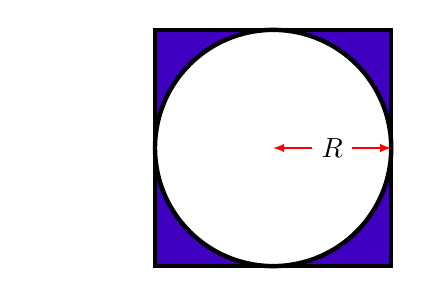
\begin{tikzpicture}[x=15mm,y=15mm,>=latex]
      \draw[black,ultra thick,fill=blue!75!red] (0,0) rectangle (2,2);
      \draw[black,ultra thick,fill=white] (1,1) circle (1);
      \draw[thin,red,<->] (1,1) -- (2,1) node[midway,black,fill=white] {$R$};
      \node at (-1,1) {\ };
    \end{tikzpicture}
  \end{minipage}
  \hfill
  \begin{minipage}{0.45\linewidth}
    \begin{align*}
      \text{A} & = \text{I have an answer}\\[0.5em]
      \text{B} & = \text{I know what to do}\\[0.5em]
      \text{C} & = \text{I am thinking}\\[0.5em]
      \text{D} & = \text{I do not know where to start}
    \end{align*}
  \end{minipage}
  \smallskip
  \pause

  \alert{Answer?}
  \pause

  The side of the square is $2R$, so the square has area $(2R)^2 =
  4R^2$.

  The area of the circle is $\pi R^2$.

  The shaded area is {\red$4R^2 - \pi R^2$}\ or {\red$(4-\pi)R^2$}.

  \begin{center}
    A$=$got it
    \quad 
    B$=$close
    \quad 
    C$=$not so close
  \end{center}

}

\frame{
  \frametitle{Review Question \#4}

  A bottle with {\blue\textsc{drink me}} written on it contains $50\%$ pure
  water and $50\%$ {\blue magicerium.} Alice wishes to add some of
  this to $7$ liters of pure water to obtain a {\red brew} which is
  $\red 20\%$ {\blue magicerium} and the rest pure water. How many
  liters should she take from the bottle labelled {\blue\textsc{drink me}}?
  \begin{center}
    A$ = 7$
    \quad 
    B$ = 14$
    \quad 
    C$ = 14/3$
    \quad 
    D$ = 7/3$
    \quad 
    E$ = 20$
    \pause
    \quad 
    \fbox{C}
  \end{center}
  \vspace*{2in}

}


\frame{
  \frametitle{Short Review Questions}

  \begin{itemize}
  \item[\red(1)]  What is the slope of the line $2y-3x=5$? 
    \begin{center}
      A$=3$
      \quad 
      B$ = -3$
      \quad 
      C$ = 2/3$
      \quad 
      D$=3/2$
      \quad 
      E$ = -3/2$
      \quad
      \pause
      \fbox{D}
    \end{center}
    \bigskip

    \item[\red(2)]  What is the $x$-coordinate of the point where the lines
      \begin{equation*}
        y+x=5
        \qquad\text{and}\qquad
        y=3x-2
      \end{equation*}
      intersect?

      \begin{center}
        A$=-1/3$
        \quad 
        B$=1/3$
        \quad 
        C$ = 3/4$
        \quad 
        D$ = 7/4$
        \quad
        \pause
        \fbox{D}
      \end{center}
      \bigskip
      
    \item[\red(3)] Solve {\Large$\frac{2^{\red x}}{3^{2{\red x}}}=5$}.
      
      \begin{center}
        A$= \log(5)/\log(2/3)$
        \quad 
        B$=\log(5)/(\log(2)-\log(3))$\\
        C$=\log(5)/(\log(2)+2\log(3))$
        \quad 
        D$=\log(5)/(\log(2)-2\log(3))$
        \quad
        \pause
        \fbox{D}
        \end{center}

  \end{itemize}

}










\end{document}

